\documentclass{beamer}
% \documentclass[11pt, handout]{beamer}

\usepackage{/home/alex/.latex/stylesheet}
\usepackage{graphicx}
\usepackage{hyperref}
\usepackage{caption}
\usepackage{subcaption}
\graphicspath{ {./images/} }

\renewcommand<>{\item}[1]{\only#2{\beameroriginal{\item}{#1}}}

\mode<presentation> {
    \usetheme{default}
    \usecolortheme{seahorse}
    \setbeamertemplate{footline}[page number] % To replace the footer line in all slides with a simple slide count uncomment this line
    \setbeamertemplate{navigation symbols}{} % To remove the navigation symbols from the bottom of all slides uncomment this line
}

\title[Short title]{Further Investigation into Schelling's Model} % The short title appears at the bottom of every slide, the full title is only on the title page
\author{Alex Ledger} % Your name
\institute[Reed College] % Your institution as it will appear on the bottom of every slide, may be shorthand to save space
{
Reed College \\ 
\medskip
\textit{aledger@reed.edu}
}
\date{\today} % Date, can be changed to a custom date

\begin{document}

\begin{frame}
    \titlepage 
\end{frame}

\begin{frame}
    \frametitle{Goal}
    I had the following questions:
    \begin{itemize}
        \item Under what conditions does Schelling's model begin to break down?
        \item Keeping the agents' preferences constant, how can we change the parameters such that the average similarity converges to difference values?
        \item What affects the the rate of convergence of the average similarity (amt. of segregation in system)?
    \end{itemize}
    My thought: let's change how the unhappy agents choose a new cell to live.
        \begin{itemize}
            \item Classically, agents move to the nearest empty cell where they would be happy.
            \item Let's try having the agents take a random walk.
        \end{itemize}
\end{frame}

\begin{frame}
    \frametitle{Recap of Schelling's Model}
    \begin{enumerate}
        \item Two types of agents (white and black) located on an $8 \times 8$ board.
            \begin{itemize}
                \item (picture a chessboard)
            \end{itemize}
        \item Each type of agent wants to have at least $x \%$ of their neighbors similar to them.
            \begin{itemize}
                \item Originally one agent wanted at least $\frac{1}{3}$ of neighbors to be similar.
                \item And the other agent wanted at least $\frac{1}{2}$ of neighbors to be similar.
            \end{itemize}
        \item If an agent's preferences are not met, then they are unhappy.
        \item During each iteration of the model, an unhappy agent is randomly selected.
        \item<1>{Then the selected agent moves to the \textbf{nearest} empty cell such that they are happy.}
        \item<2>{\color[rgb]{0,0,1} Then the selected agent moves to the \textbf{nearest} empty cell such that they are happy.}
        \item<3>{\color[rgb]{0,0,1} Then the selected agent searches for a new cell where they would be happy via a \textbf{random walk}.}
    \end{enumerate}
\end{frame}

\begin{frame}
    \frametitle{What is a random walk?}
    \begin{itemize}
        \item After an agent is selected to move, the agent randomly selects a direction that they could move.
            \begin{itemize}
                \item e.g. North, South, East West (updated appropriately at borders)
            \end{itemize}
        \item The agent then ``moves'' to the cell adjacent to their current position in the selected direction.
        \item If the cell is empty and the agent is happy, then the agent ``settles'' in the cell and turn is over.
        \item Otherwise the agent randomly selects a direction and moves to that cell, repeating the above steps.
        \item Eventually the agent will either find a cell they like, or will have taken more than $100$ steps. 
        \item If the agent takes more than $100$ steps, they return to their original cell and their turn is over.
    \end{itemize}
\end{frame}

\begin{frame}[t]
    \frametitle{Example of a Random Walk}

    Suppose that {\color[rgb]{.34,.34,.34} W} is selected to move and wants $\geq \frac{1}{2}$ of neighbors to also be white. \\
    \begin{columns}[t,onlytextwidth]

    \column{.5\textwidth}
    \begin{figure}
        \center
        The Random Walk:
        \begin{enumerate}
            \item Goes East.
            \item Goes South.
            \item Goes West.
            \item Finds empty and happy cell. 
        \end{enumerate}
    \end{figure}

    \column{.5\textwidth}
        \begin{figure}
            \center
            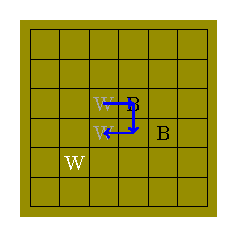
\includegraphics[scale=1.2]{random_walk/random_walk.pdf}
        \end{figure}
    \end{columns}
\end{frame}

\begin{frame}
    \frametitle{Measuring a state in Schelling's model}
    We can measure a state by measuring the \emph{average similarity} or the \emph{average happiness}.
    \begin{align*}
        \text{Similarity(agent)} & = \frac{\text{\# neighbors of agent's race}}{\text{\# of neighbors}} \\
        \\
        \text{Similarity(state)} & = \text{Average similarity of all agents} \\
        \\
        \text{Happiness(state)}  & = \frac{\text{\# happy agents}}{\text{\# total agents}} 
    \end{align*}
    Similarity gives you the amount of segregation in the system.

        

    \end{frame}

\begin{frame}
    \frametitle{Results}

    \begin{columns}[t,onlytextwidth]

        
    \column{.3\textwidth}
        \footnotesize
        \begin{itemize}
            \item Initialize a random state.
            \item Run the model 50 iterations.
            \item Record average similarity and average happiness at each iteration.
            \item Ran 25 trials and plotted averages (see right).
            \item The nearest and rw trials used the same initial states.
        \end{itemize}
        \normalsize

    \column{.6\textwidth}
        \begin{figure}[t]
            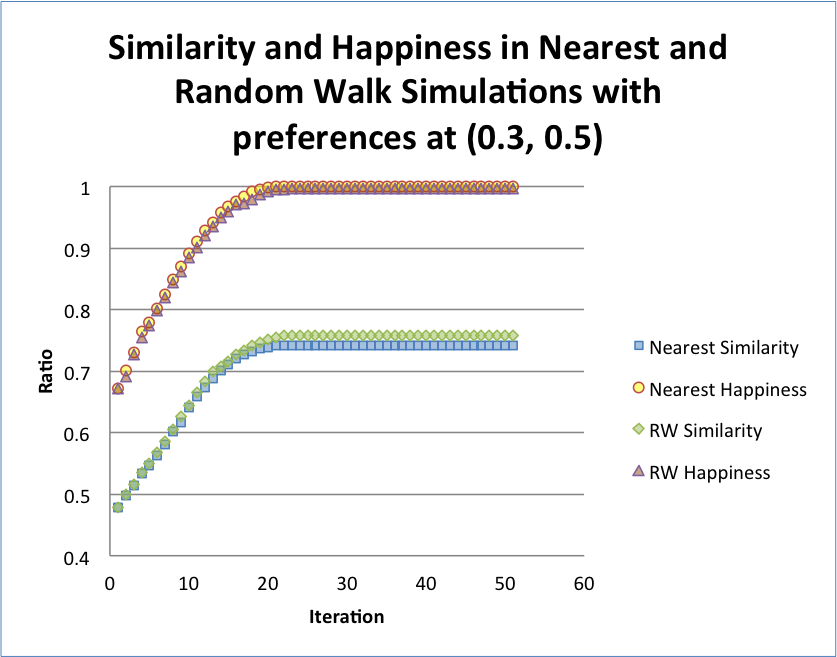
\includegraphics[scale=0.5]{data_images/3_5.png}
        \end{figure}

    \end{columns}
\end{frame}


\begin{frame}
    \vspace{-15.5pt}
    \begin{columns}[t,onlytextwidth]

    \column{.1\textwidth}
    \begin{figure}
        \begin{subfigure}[b]{0.3\textwidth}
            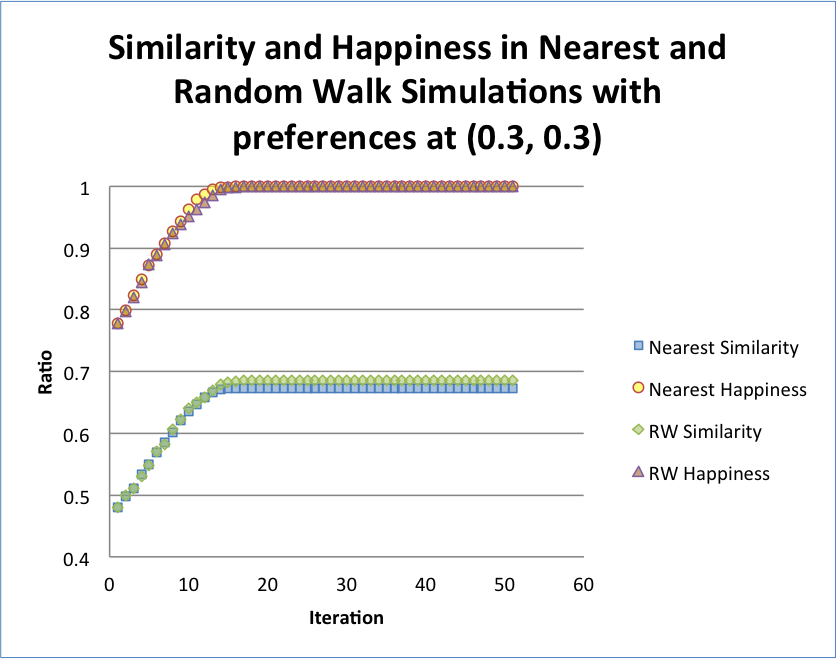
\includegraphics[scale=0.35]{data_images/3_3.png}
        \end{subfigure}

        \begin{subfigure}[b]{0.3\textwidth}
            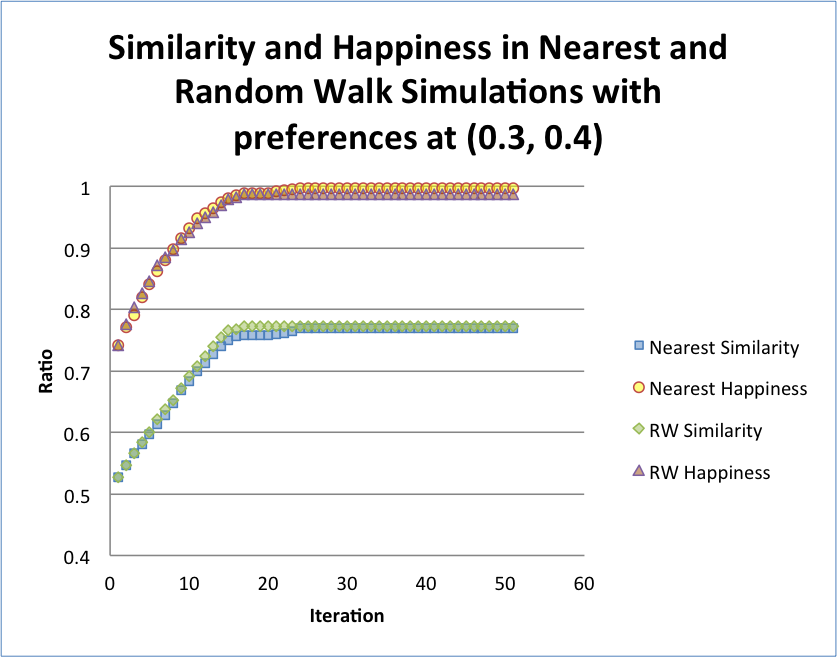
\includegraphics[scale=0.35]{data_images/3_4.png}
        \end{subfigure}
    \end{figure}

    \column{.7\textwidth}
    \begin{figure}
        \begin{subfigure}[b]{0.3\textwidth}
            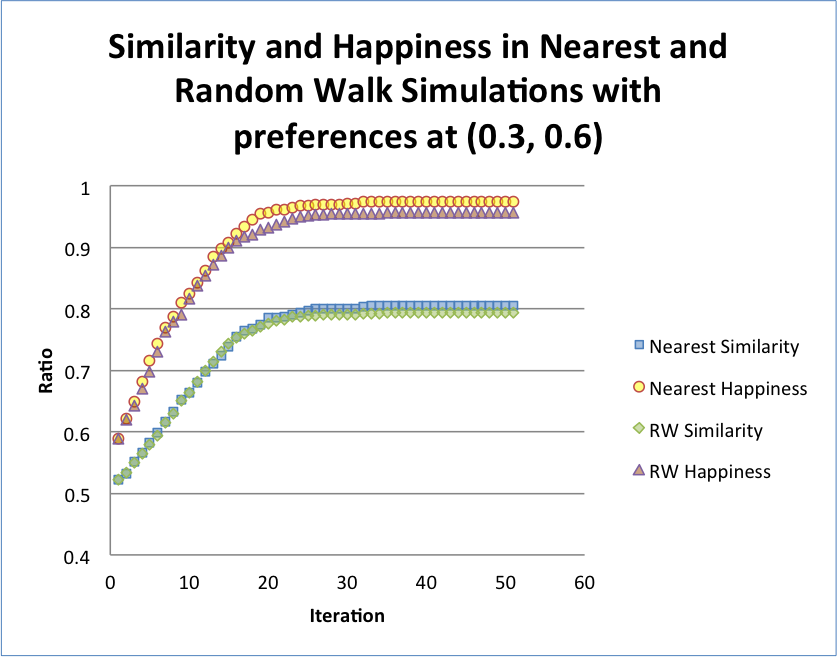
\includegraphics[scale=0.35]{data_images/3_6.png}
        \end{subfigure}

        \begin{subfigure}[b]{0.3\textwidth}
            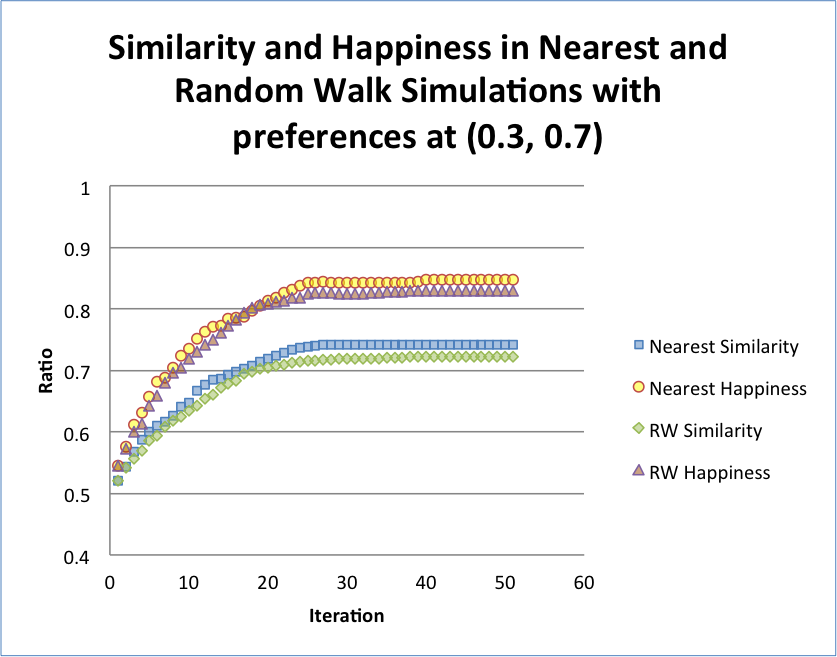
\includegraphics[scale=0.35]{data_images/3_7.png}
        \end{subfigure}
    \end{figure}
    \end{columns}
\end{frame}

\begin{frame}
    \frametitle{Analysis of the model}
    So unfortunately, I didn't find any parameters for which the nearest model and random walk model exhibited different behavior.
    \\
    Ideas for further investigation:
    \begin{itemize}
        \item Change max number of number steps an agent can take in their random walk.
        \item Change border conditions (in particular, make the border a torus instead of an edge)
        \item Inspired by Zach's talk: every $x$ iterations, force a happy person to move at least $y$ cells away from their place.  
        \item Try modeling socioeconomic inequality by giving agents a certain amount of steps they can take in their random walk (give some agents more steps than others).
        \item Try reversing Schelling's model. Instead of agent's desiring a particular composition of neighbors, neighbors have a desire about whether or not they want to live by you. 
            \begin{itemize}
                \item Would perhaps model living near sex offenders/felons/sexism - phenomena with outward effects
            \end{itemize}
    \end{itemize}
\end{frame}

\begin{frame}
    \frametitle{Philosophical Analysis}
    \footnotesize
    Other goal: To what extent can we make conclusions about society based on knowledge gained from Schelling's model?
    \begin{itemize}
        \footnotesize
        \item Since Schelling's model is a huge simplification of reality, it's arguable whether the results translate to society.
        \item My thought: let's make Schelling's model a tiny bit more realistic and see what happens.
            \begin{itemize}
                \scriptsize
                \item I think adding the random walk is a \emph{huge} change to Schelling's model.
                    \begin{itemize}
                        \scriptsize
                        \item The model is no longer nondeterministic
                        \item etc. 
                    \end{itemize}
                \end{itemize}
        \item We saw: results were the same.
        \item What it suggests: 
            \begin{itemize}
                \scriptsize
                \item The core component of Schelling's model (preferences/racism and happiness) is robust.
                \item Changing the procedure around the core doesn't seem to change much about the model.
                \item Suggests to me that the mechanism is secondary to the phenomon
                \item i.e. how we react to racism is secondary to the existence of racism.
            \end{itemize}
    \end{itemize}
\end{frame}

\begin{frame}
    \frametitle{The Upshot}
    \begin{itemize}
        \item Need to do more work.
        \item Tentative thinking: the random walk does not break Schelling's model
        \item So the ``core'' idea of Schelling's model is robust.
        \item ``core'' idea = preferences/happiness
        \item ``non-core'' idea = movement procedure
    \end{itemize}
\end{frame}


\end{document} 






































